\documentclass[11pt,a4paper]{article} 

% Define page geometry
\usepackage{geometry}
\geometry{left=2.2cm,
	right=2.2cm,
	top=2.2cm,
	bottom=2cm} % Page margins
\parskip 0.15cm % Paragraph spacing
\setlength{\parindent}{0cm} % No paragraph indenting

% Text formatting
\usepackage[T1]{fontenc} % Set font
\usepackage{lineno} % Line numbers
\linespread{1.5} % Linespacing

\usepackage{amssymb}
\usepackage{multirow}
\setlength{\tabcolsep}{4pt} % Default table column sep width 

\usepackage{fmtcount}

% Image handling
\usepackage{graphicx} 
\graphicspath{ {img/} } % Define image path
\usepackage{float} % Precise figure location

% Bibliography management
\usepackage[natbib, 
	style=authoryear, 
	uniquename=false, 
	uniquelist=false,
	giveninits=true,
	dashed=false,
	maxcitenames=2, 
	mincitenames=1, 
	minbibnames=10, 
	maxbibnames=10, 
	backend=biber]{biblatex}
\renewcommand*\finalnamedelim{\addspace\&\space}
\addbibresource{phenology.bib}

% Links within document, nice figure formatting
\usepackage{xcolor}
\usepackage[breaklinks]{hyperref}
\definecolor{links}{RGB}{0,0,0}
\hypersetup{
	breaklinks,
	colorlinks=true,
	linkcolor=links,
	anchorcolor=links,
	citecolor=links,
	filecolor=links,
	menucolor=links,
	runcolor=links,
	urlcolor=links,
	pdfauthor={John L. Godlee}
}
\def\subsectionautorefname{section}
\def\subsubsectionautorefname{section}

\newcommand{\beginsupplement}{%
	\setcounter{table}{0}
	\renewcommand{\thetable}{S\arabic{table}}%
	\setcounter{figure}{0}
	\renewcommand{\thefigure}{S\arabic{figure}}%
	}
   
% Variables
\newcommand{\censusDate}{2014}
\newcommand{\nTotalSites}{993}
\newcommand{\modisSLC}{0.05}
\newcommand{\trmmSLC}{0.06}
\newcommand{\plotDistPer}{93.9}
\newcommand{\nscaInertia}{1.81}
\newcommand{\mopanePer}{50}
\newcommand{\stemsHa}{50}
\newcommand{\stemSize}{10}
\newcommand{\nSites}{709}


\begin{document}

{\Large{Title: Diversity and woodland structure mediate land-surface phenology in Zambia}}

Authors: Godlee J. L.\textsuperscript{1}, Ryan C. M.\textsuperscript{1}, Siampale A.\textsuperscript{2}, Dexter K. G.\textsuperscript{1,3}

\textsuperscript{1}School of GeoSciences, University of Edinburgh, Edinburgh, EH9 3FF, United Kingdom \\
\textsuperscript{2}Forestry Department Headquarters - Ministry of Lands and Natural Resources, Cairo Road, Lusaka, Zambia \\
\textsuperscript{3}Royal Botanic Garden Edinburgh, Edinburgh, EH3 5LR, United Kingdom \\

\vspace{1em}
Corresponding author:

John L. Godlee

johngodlee@gmail.com

School of GeoSciences, University of Edinburgh, Edinburgh, United Kingdom

\section*{Acknowledgements}

\section*{Author contribution statement}

JLG conceived the study, conducted the analysis, and wrote the first draft of the manuscript. AS coordinated plot data collection in Zambia, and initial data management. All authors contributed to manuscript revisions. 

\section*{Data accessibility statement}

The data used in this study are held by the Zambian Integrated Land Use Assessment Project (ILUA-II), and were cleaned by the SEOSAW project (Socio-Ecological Observatory for Southern African Woodlands). An anonymised version of the plot data are available at the following DOI: .

\newpage{}
\linenumbers

\section*{Abstract}

Land-surface phenology is a key determinant of ecosystem function across the dry tropics, and measures of land-surface phenology are routinely included in earth system models to constrain estimates of productivity. Future variation in phenology can be predicted to some extent from climatic variables, but our understanding of how ecosystem structure mediates variation in phenology is lacking, commonly limited to coarse plant functional types. We combined a dense plot network of 672 sites across deciduous Zambian woodlands with remotely sensed land-surface phenology metrics to investigate the role of tree species diversity, composition, and demographic structure on phenology, including the phenomenon of pre-rain green-up. We found positive effects of tree species diversity on season length and pre-rain green-up, variation among miombo and non-miombo vegetation types in their phenological patterns and biotic drivers of phenology, and a strong effect of large trees as drivers of the pre-rain green-up and senescence lag effects. The study exemplifies the role of biotic diversity as a determinant of ecosystem function, and offers new insights into the factors which determine land-surface phenology across the dry tropics, which can inform earth system modelling approaches.

\section{Introduction}

The seasonal timing and duration of foliage production (land-surface phenology) is a key mediator of land-atmosphere exchanges. Foliage forms the primary interface between plants, the atmosphere and sunlight \citep{Gu2003, Penuelas2009}, thus land-surface phenology plays an important role in regulating global carbon, water and nitrogen cycles \citep{Richardson2013}. Carbon-cycling models routinely incorporate land-surface phenological processes, most commonly through remotely-sensed data products (e.g. \citealt{Bloom2016}), but our understanding of the ecological mechanisms which determine these phenological processes remains under-developed \citep{Whitley2017}. This limits our ability to predict how land-surface phenology will respond to climate and biodiversity change, and how these responses will vary among species and vegetation types \citep{Xia2015}.

At regional scales, land-surface phenology can be predicted using only climatic factors, namely precipitation, diurnal temperature, and light environment \citep{Adole2018a}, but significant local variation exists within biomes in the timing of leaf production which cannot be attributed solely to abiotic environment \citep{Stockli2011}. It has been repeatedly suggested that the diversity, composition, and demographic structure of plant species plays a role in determining how ecosystems respond to abiotic phenological cues \citep{Adole2018b, Jeganathan2014, Fuller1999}, owing to differences in life history strategy among species and demographic groups, but current implementation of biotic variation in earth system models is often limited to coarse plant functional types, which are unable to represent the wide variation in phenological patterns observed at local scales \citep{Scheiter2013, Pavlick2013}.

Across the dry tropics, seasonal oscillations in water availability produce strong cycles of foliage production \citep{Chidumayo2001, Dahlin2016}, with knock-on effects for ecosystem function. The phenomenon of pre-rain green-up seen in some tree species within the dry tropics serves as a striking example of adaptation to seasonal variation in water availability \citep{Ryan2017}. Conservative species, i.e. slower growing, with robust leaves and denser wood, may initiate leaf production (green-up) before the wet season has commenced. More acquisitive species and juveniles however, tend to green-up during the wet season creating a dense leaf-flush during the mid-season peak of growth and dropping their leaves earlier as the wet season ends. Both strategies have associated costs and benefits which allow coexistence of species exhibiting a range of phenological syndromes along this spectrum. While conservative species gain a competitive advantage from having fully emerged leaves when the wet season starts, they must also invest heavily in deep root architecture to access dry season groundwater reserves in order to produce foliage during the dry season. Similarly, while acquisitive species minimise the risk of hydraulic failure and mortality by only producing leaves when conditions are amenable, they forfeit growing season length. It has been suggested that variation in phenological strategy among tree species is one mechanism by which increased species diversity increases resilience to drought and maximises productivity in water-limited woodland ecosystems \citep{Stan2019, Morellato2016}. By providing functional redundancy within the ecosystem, leaf production can be maintained under a wider range of conditions, therefore maximising long-term productivity.

In addition to determining productivity, variation in leaf phenology also affects broader ecosystem function. Woodlands with a longer tree growth period support a greater diversity and abundance of wildlife, particularly birds, but also browsing mammals and invertebrates \citep{Cole2015, Araujo2017, Morellato2016, Ogutu2013}. As climate change increases the frequency and severity of drought in water-limited woodlands, it is feared that this will result in severe negative consequences for biodiversity \citep{Bale2002}. The periods of green-up and senescence which bookend the growing season are key times for invertebrate reproduction \citep{Prather2012} and herbivore browsing activity \citep{Velasque2016, Morellato2016}. Pre-rain green-up provides a valuable source of moisture and nutrients before the wet season, and can moderate the understorey microclimate, increasing humidity, reducing UV exposure, and moderating diurnal oscillations in temperature, reducing ecophysiological stress which can lead to mortality during the dry season. Additionally, a slower rate of green-up caused by tree species greening at different times, i.e. reduced synchronicity, provides an extended period of bud-burst, maintaining the important food source of nutrient rich young leaves for longer. Thus, understanding the determinants of seasonal patterns of tree leaf production in dry deciduous woodlands can provide valuable information on spatial variation in vulnerability to climate change, and help to model their contribution to earth system models under climate change.
 
In this study we investigated how tree species diversity, composition, and demographic structure influence three key measurable aspects of the tree phenological cycle of dry tropical woodlands: (1) the lag time between green-up/senescence and the start/end of the wet season, (2) the rates of greening and senescence at the start and end of the seasonal growth phase, and (3) the overall length of the growth period. We hypothesise that: (H\textsubscript{1}) sites with greater species diversity will exhibit a longer growth period and greater cumulative green-ness over the course of the growth period, due to a higher resilience to variation in water availability. Additionally, we hypothesise that: (H\textsubscript{2}) in sites with greater species diversity the start of the growing season will occur earlier with respect to the onset of rain due to an increased likelihood of containing a species which can green-up early, and that (H\textsubscript{3}) due to variation among species in phenological strategy and minimum water requirement, sites with greater tree species diversity will exhibit slower rates of greening and senescence as different species green-up and senesce at different times. We hypothesise that: (H\textsubscript{4}) irrespective of species diversity, variation in tree species composition and vegetation type will cause variation in the phenological metrics outlined above. Finally, we hypothesise that: (H\textsubscript{5}) sites with larger trees will exhibit earlier pre-rain green-up and later senescence, under the assumption that large trees can better access resilient deep groundwater reserves outside of the wet season.

\section{Materials and methods}

\subsection{Plot data}

We used data on tree species diversity and composition across \nSites{} sites from the Zambian Integrated Land Use Assessment Phase II (ILUA-II), conducted in \censusDate{} \citep{Mukosha2009, Pelletier2018}. Each site consisted of four 20x50 m (0.1 ha) plots positioned in a square around a central point, with a distance of 500 m between each plot (\autoref{schematic}). The original census contained \nTotalSites{} sites, which was filtered in order to define study bounds and to ensure data quality. Only sites with $\geq$\treesHa{} stems ha\textsuperscript{-1} $\geq$\stemSize{} cm DBH (Diameter at Breast Height) were included in the analysis, to ensure all sites represented woodlands rather than `grassy savanna', which is considered a separate biome with different species composition and ecosystem processes governing phenology \citep{Parr2014}. Sites dominated by non-native tree species ($\geq$50\% of individuals), e.g. \textit{Pinus} spp. and \textit{Eucalyptus} spp. were excluded, as these species may exhibit non-seasonal patterns of foliage production \citep{Broadhead2003}. Of the \nTrees{} trees recorded, \perSpIndet{}\% were only identified to genus, and \perGenIndet{}\% could not be identified.

\begin{figure}[H]
\centering
	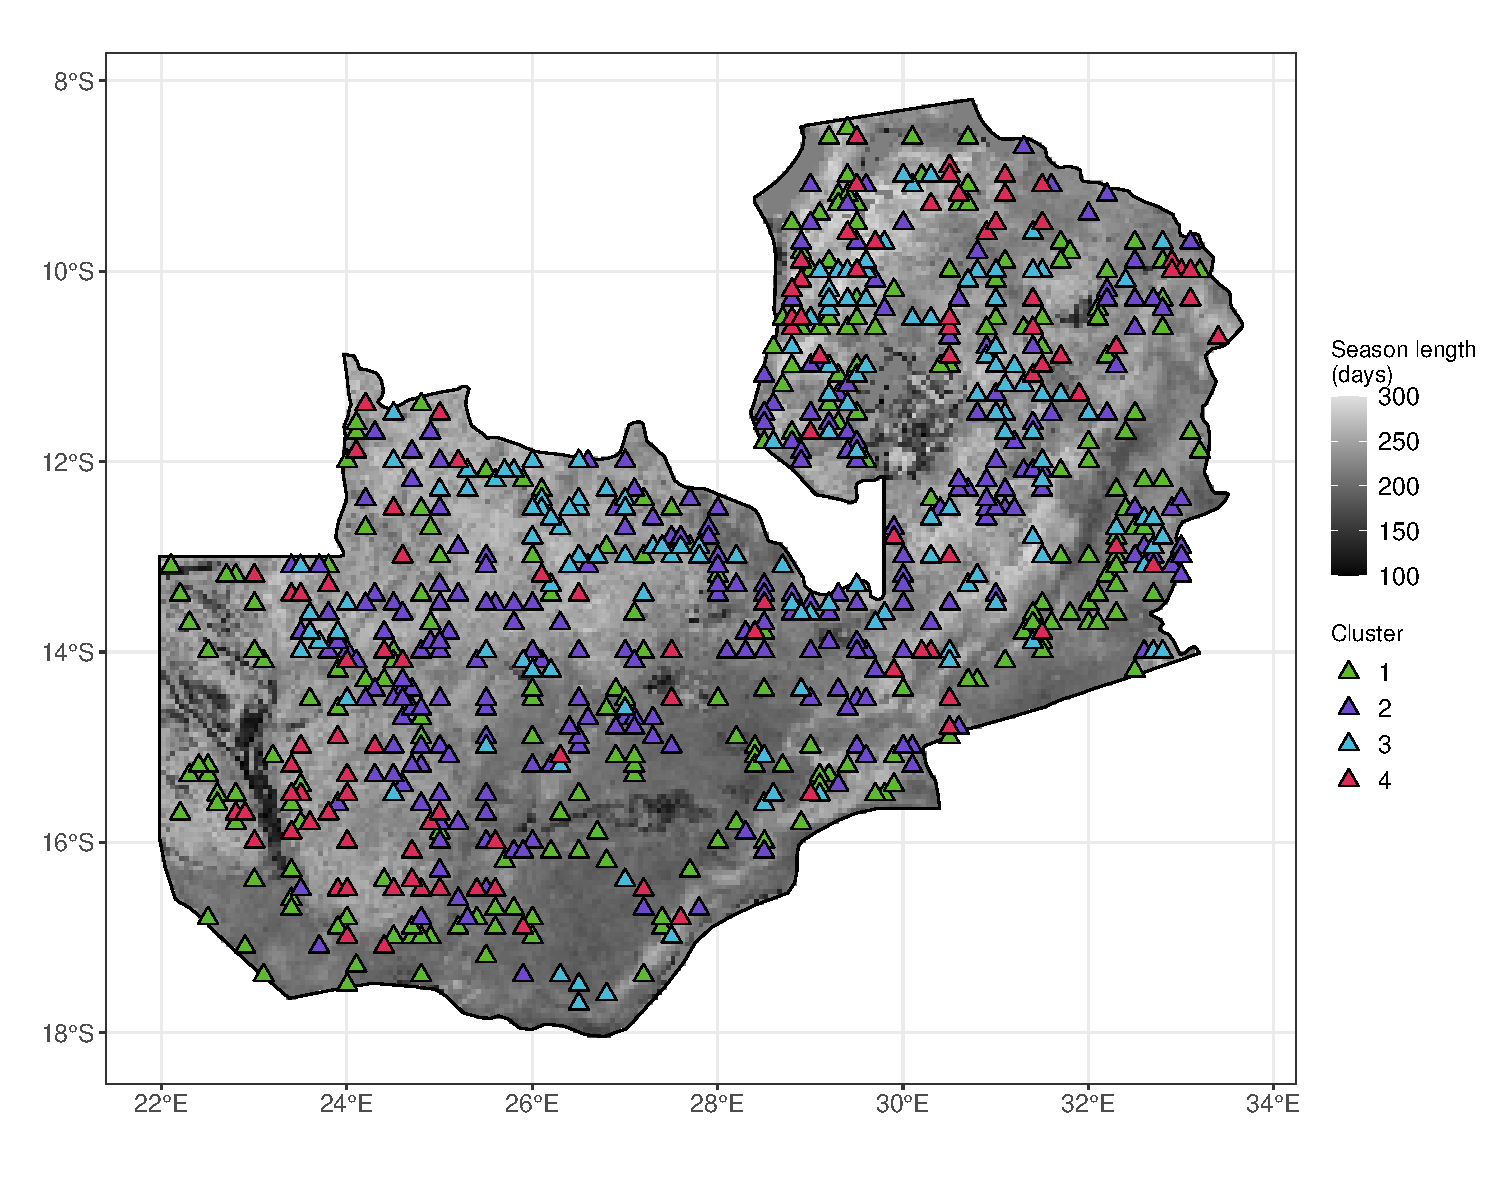
\includegraphics[width=0.8\textwidth]{plot_loc}
	\caption{Distribution of study sites within Zambia as triangles, each consisting of four plots. Sites are coloured according to vegetation compositional cluster as identified by Ward's clustering algorithm on the Bray-Curtis distance of plots by species basal area. Zambia is shaded according to growing season length as estimated by the MODIS VIPPHEN-EVI2 product, at 0.05\textdegree{} spatial resolution \citep{VIPPHEN}.}
	\label{plot_loc}
\end{figure}

\begin{figure}[H]
\centering
	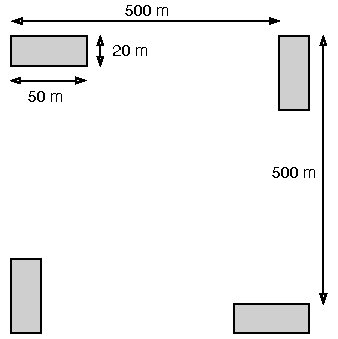
\includegraphics[width=0.5\textwidth]{schematic}
	\caption{Schematic diagram of plot layout within a site. Each 20x50 m (0.1 ha) plot is shaded grey. Note that the plot dimensions are not to scale.}
	\label{schematic}
\end{figure}

Within each plot, the species of all trees with at least one stem $\geq$\stemSize{} cm DBH were recorded. Plot data was aggregated to the site level for analyses to avoid pseudo-replication caused by the more spatially coarse phenology data. Tree species composition varied little among the four plots within a site, and were treated as representative of the woodland in the local area. Using the Bray-Curtis dissimilarity index on species basal area data \citep{Faith1987}, we calculated that the mean pairwise compositional distance between plots within a site was lower than the mean compositional distance across all pairs of plots in \plotDistPer{}\% of cases.

\subsection{Plot data analysis} 

To measure variation in tree species composition we used agglomerative hierarchical clustering on species basal area data \citep{Kreft2010, Fayolle2014}. To guard against sensitivity to rare individuals, which can preclude meaningful cluster delineation across such a large species compositional range, we excluded species with less than five records, and restricted the dataset to sites with more than five species. We used Ward's algorithm to define clusters \citep{Murtagh2014}, based on the Bray-Curtis distance of sites. We determined the optimal number of clusters by maximising the mean silhouette width among clusters \citep{Rousseeuw1987}. Vegetation type clusters were used later as interaction terms in linear models. We described the vegetation types represented by each of the clusters using a Dufrene-Legendre indicator species analysis \citep{Dufrene1997}.

To describe the species diversity of each site, we calculated the Shannon-Wiener index ($H'$) from species basal area rather than individual abundance, as a measure of species diversity effectively weighted by a species' contribution to canopy occupancy and thus by contribution to the phenological signal. $H'$ was transformed to the first order numbers-equivalent ($^1\!D$) of $H'$, calculated as $e^{H'}$ \citep{Jost2007}. We use $^1\!D$ as the primary measure of species diversity in our statistical models, and is subsequently referred to as species diversity. Additionally, we calculated a separate measure of abundance evenness, using the Shannon Equitability index ($E_{H'}$) \citep{Smith1996}. $E_{H'}$ was calculated as the ratio of basal area Shannon-Wiener diversity index to the natural log of total basal area per site. To describe average tree size, we calculated the quadratic mean of stem diameters per site \citep{Curtis2000}. The quadratic mean gives more weight to large trees and is thus more appropriate for our use, where we are interested in the contribution of large trees to land-surface phenology. 

\subsection{Land-surface phenology data}

To quantify phenology at each site, we used the MODIS MOD13Q1 satellite data product at 250 m resolution \citep{MOD13Q1}. The MOD13Q1 product provides an Enhanced Vegetation Index (EVI) time series at 16 day intervals. EVI is widely used as a measure of vegetation growth and is well-correlated with Gross Primary Productivity (GPP), thus providing a measure of land-surface phenology that is relevant to carbon cycling \citep{Sjostrom2011}. We used all scenes from January 2010 to December 2020 with less than 20\% cloud cover covering the study area. All sites were determined to have a single annual growth season according to the MODIS VIPPHEN product \citep{VIPPHEN}, which assigns pixels (0.05\textdegree, 5.55 km at equator) up to three growth seasons per year. We stacked yearly data between 2010 and 2020 and fit a General Additive Model (GAM) to produce an average EVI curve (\autoref{ts_example}). We estimated the start and end of the growing season using first derivatives of the GAM. The start of the growing season was identified as the first day where the model slope exceeds half of the maximum positive model slope for a continuous period of \modisWin{} or more days, using only backwards looking data, following \citet{White2009}. Similarly, we defined the end of the growing season as the final day of the latest \trmmWin{} period where the GAM slope meets or exceeds half of the maximum negative slope. We estimated the length of the growing season as the number of days between the start and end of the growing season. We calculated cumulative EVI as the EVI accumulated over the growing season, and is reported in the results divided by 100000. We estimated the green-up rate as the slope of a linear model across EVI values between the start of the growing season and the point at which the slope of reduces below half of the maximum positive slope. Similarly the senescence rate was estimated as the slope of a linear model between the latest point where the slope of decrease fell below half of the maximum negative slope and the end of the growing season. We validated our calculations of cumulative EVI, mean annual EVI, growing season length, season start date, season end date, green-up rate and senescence rate with calculations made by the MODIS VIPPHEN product with linear models comparing the two datasets across our study sites (\autoref{vipphen_compare}, \autoref{annot_df}). We chose not to use the MODIS VIPPHEN product directly due to its more coarse spatial resolution (0.05\textdegree, 5.55 km at equator).

Precipitation data was gathered using the ``GPM IMERG Final Precipitation L3 1 day V06'' dataset, which has a pixel size of 0.1\textdegree (11.1 km at the equator) \citep{IMERG}, between 2010 and 2020. Daily total precipitation was separated into three periods: precipitation during the growing season (wet season precipitation), precipitation in the 90 day period before the onset of the growing season (pre-green-up precipitation), and precipitation in 90 day period before the onset of senescence at the end of the growing season (pre-senescence precipitation). Wet season limits were defined as for the EVI data, using the first derivative of a GAM to create a curve for each site using stacked yearly precipitation data, from which we estimated the half-maximum positive and negative slope to identify where the GAM model exceeded these slope thresholds for a consistent period of 20 days or more. Mean diurnal temperature range (Diurnal $\delta$T) was calculated as the mean of monthly temperature range from the WorldClim database, using the BioClim variables, with a pixel size of 30 arc seconds (926 m at the equator) \citep{Fick2017}, averaged across all years of available data (1970-2000). We calculated the lag between the onset of the growing season and the onset of the wet season as the difference between these two dates as calculated above. We performed a similar calculation to estimate the lag between the end of the growing season and the end of the wet season. 

\begin{figure}[H]
\centering
	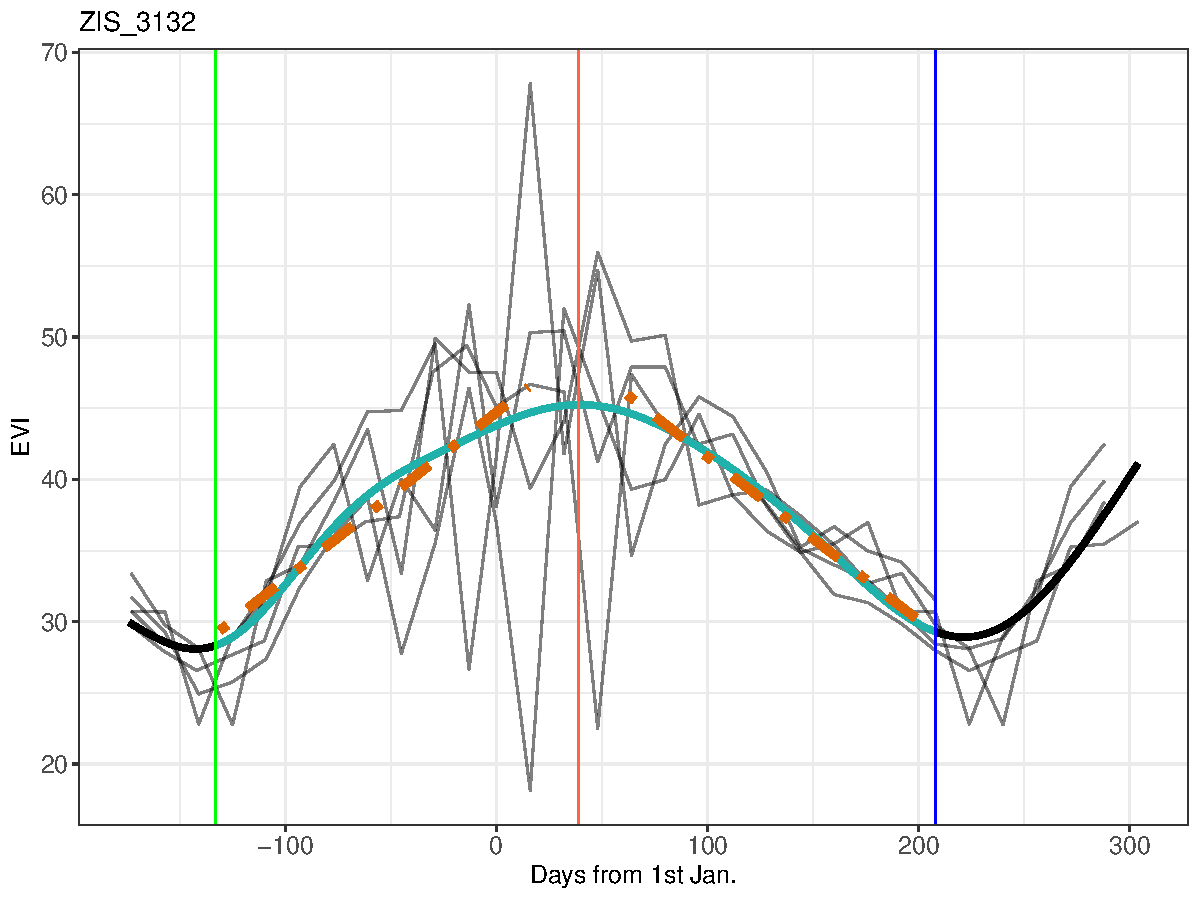
\includegraphics[width=0.8\textwidth]{ts_example}
	\caption{Example EVI time series, demonstrating the metrics derived from it. Thin black lines show the raw EVI time series, with one line for each annual growth season. The thick black line shows the GAM fit. The thin blue lines show the minima which bound the growing season. The red line shows the maximum EVI value reached within the growing season. The shaded cyan area of the GAM fit shows the growing season, as defined by the first derivative of the GAM curve. The two orange dashed lines are linear regressions predicting the green-up rate and senescence rate at the start and end of the growing season, respectively. Note that while the raw EVI time series fluctuate greatly around the middle of the growing season, mostly due to cloud cover, the GAM fit effectively smooths this variation to estimate the average EVI during the mid-season period.}
	\label{ts_example}
\end{figure}

\subsubsection{Statistical modelling}

We used linear mixed effects models to assess the role of tree species diversity on each phenological metric. We defined a maximal model structure including the fixed effects of species diversity and evenness, alongside climatic variables shown by previous studies to strongly influence land-surface phenology, with vegetation cluster as a random slope effect on species diversity. The maximal model was compared to models with different subsets of fixed effects using the model log likelihood, AIC (Akaike Information Criteria), BIC (Bayesian Information Criteria), and adjusted R\textsuperscript{2} values for each model, to determine which combination of fixed effects best explained each phenological metric. Where two similar models were within 2 AIC points of each other, the model with fewer terms was chosen as the best model, to maximise model parsimony. All models were fitted using Maximum Likelihood (ML) to allow comparison of models with different fixed effects \citep{Zuur2009}. The best model was subsequently re-fitted using Restricted Maximum Likelihood (REML) for model effect size estimation. Fixed effects in each model were transformed to achieve normality where necessary and standardised to Z-scores prior to modelling to allow comparison of slope coefficients within a given model.

We used the \texttt{ggeffects} package to estimate the marginal means of the effect of species diversity on each phenological metric among vegetation clusters \citep{ggeffects}. Estimating marginal means entails generating model predictions across values of a focal variable, in this case species diversity, while holding non-focal variables constant at their reference value. All statistical analyses were conducted in R version 4.0.2 \citep{R2020}.

To investigate the effect of tree size on each phenological metric, we conducted a separate set of linear mixed effects models, including the fixed effect of tree size and vegetation cluster as a random intercept term. We used fixed effect sizes to determine the effect of tree size on each phenological metric.

To describe variation within and among vegetation clusters in their land-surface phenology we conducted a simple MANOVA using the phenological metrics as response variables, followed by post-hoc Tukey's tests between each pairwise combination of vegetation clusters per phenological metric, to test whether vegetation clusters differed significantly in their land-surface phenology.

\section{Results}

Model selection showed that both diversity and evenness were significant fixed effects in models predicting cumulative EVI, season length, and green-up lag (\autoref{mod_slopes}), while senescence rate, senescence lag, and green-up rate were poorly predicted across all our models (\autoref{mod_stat}). As expected (H\textsubscript{1}), species diversity and wet season precipitation both had positive significant effects on cumulative EVI and season length. In contrast, abundance evenness, the other aspect of tree species diversity in our models, had a significant negative effect on both cumulative EVI and season length (\autoref{mod_slopes}).

Species diversity caused a significant increase in the green-up lag, i.e. the length of the period between green-up and wet season onset (H\textsubscript{2}). This effect was comparable to the effects of pre-green-up precipitation and diurnal temperature range, which also caused an increase in green-up lag (\autoref{mod_stat}). The best model predicting green-up lag explained 34\% of the variance in this phenological metric. In contrast, senescence lag was poorly defined by our models. The effects of diurnal temperature range and wet season precipitation had wide confidence intervals in the best model for senescence lag, and explained only 8\% of the variance in senescence lag. Green-up and senescence rates (H\textsubscript{3}) were also poorly constrained in our models, with neither of the best models being appreciably better than a climate only model according to AIC (\autoref{mod_stat}), and only explaining 18\% and 15\% of the variance in these phenological metrics, respectively.

\Numberstringnum{\nCluster} vegetation type clusters were identified during hierarchical clustering. The silhouette value of the clustering algorithm reached \silBest{}. Cluster 2, consists of small stature Zambesian woodlands, as referenced by \citet{Dinerstein2017} and \citet{Chidumayo2001}, and is not dominated by a particular large canopy tree species. It is possible that these woodlands represent highly disturbed miombo woodlands where large trees may have been removed by humans, or alternatively represent resource-limited woodlands due to their low precipitation. Clusters 1, 3 and 4 represent varieties of miombo woodland, dominated by \textit{Brachystegia} spp. and \textit{Julbernardia} spp., with different secondary species. Median species richness is similar across vegetation clusters (\autoref{clust_summ}).

The slope of the relationship between species diversity and phenological metrics varied among vegetation clusters (H\textsubscript{4}) (\autoref{mod_marg}). According to post-hoc Tukey's tests on marginal effects, Cluster 2 differed from all other clusters in the effect of species diversity on cumulative EVI and season length, and differed from Cluster 1 in the effect of species diversity on green-up lag. The effect of species diversity on green-up lag remained strongly similarly positive across all vegetation clusters. The effect of species diversity in Clusters 1, 3 and 4 did not differ significantly for any other phenological metric (\autoref{lsq_terms}).  

Clusters, 1, 3 and 4 were largely similar in their density distribution of the six phenological metrics, while Cluster 2 had more plots with lower cumulative EVI and lower season length \autoref{phen_dens_clust}. A MANOVA including all phenological metrics showed a significant difference among vegetation clusters (\phenManova{}). Post-hoc Tukey's tests showed significant differences between Cluster 2 and the other three clusters for all phenological metrics (\autoref{tukey_terms}). There was little spatial structure to the vegetation clusters identified (\autoref{plot_loc}). The key emergent trends were that Cluster 1 was largely absent from the southwest of the country. Cluster 4 dominated the southwest of the country, possibly representing drier Angolan miombo woodland. 

Average tree size, measured by the quadratic mean of stem DBH, caused a greater degree of pre-rain green-up, and also increased the growing season beyond the end of the wet season (H\textsubscript{5}, \autoref{diam_quad_mod_slopes}). None of the other phenological metrics were significantly affected by average tree size.

% latex table generated in R 4.0.2 by xtable 1.8-4 package
% Tue Nov 10 17:13:14 2020
\begin{table}[H]
\centering
\begin{tabular}{ccccccc}
  \hline
Cluster & N sites & Richness & MAP & Diurnal $\delta$T & Species & Indicator value \\ 
  \hline
 &  &  &  &  & \textit{Julbernardia paniculata} & 0.712 \\ 
  1 & 91 & 13(6) & 966(139.7) & 14(1.3) & \textit{Psuedolachnostylis maprouneifolia} & 0.222 \\ 
   &  &  &  &  & \textit{Pericopsis angolensis} & 0.209 \\ 
   \hline
 &  &  &  &  & \textit{Brachystegia boehmii} & 0.764 \\ 
  2 & 127 & 16(6) & 1054(162.5) & 13(1.5) & \textit{Psuedolachnostylis maprouneifolia} & 0.234 \\ 
   &  &  &  &  & \textit{Uapaca kirkiana} & 0.227 \\ 
   \hline
 &  &  &  &  & \textit{Pterocarpus angolensis} & 0.333 \\ 
  3 & 487 & 15(7) & 1037(195.9) & 14(1.6) & \textit{Brachystegia spiciformis} & 0.318 \\ 
   &  &  &  &  & \textit{Diplorhynchus condylocarpon} & 0.298 \\ 
  \end{tabular}
\caption{Climatic information and Dufrene-Legendre indicator species analysis for the vegetation type clusters identified by the PAM algorithm, based on basal area weighted species abundances. The three species per cluster with the highest indicator values are shown along with other key statistics for each cluster. MAP (Mean Annual Precipitation) and Diurnal $\delta$T are reported as the mean and 1 standard deviation in parentheses. Species richness is reported as the median and the interquartile range in parentheses.} 
\label{clust_summ}
\end{table}



% latex table generated in R 4.0.2 by xtable 1.8-4 package
% Sat Oct 31 12:21:16 2020
\begin{table}[H]
\centering
\begin{tabular}{rcccc}
  \hline
Response & $\delta$AIC & $\delta$BIC & R\textsuperscript{2}\textsubscript{adj} & $\delta$logLik \\ 
  \hline
Cumulative EVI & 43.1 & 34.0 & 0.34 & -23.54 \\ 
  Season length & 25.9 & 21.4 & 0.17 & -13.97 \\ 
  Green-up rate & 8.1 & 3.6 & 0.10 & -5.07 \\ 
  Senescence rate & 10.1 & 1.0 & 0.03 & -7.04 \\ 
  Green-up lag & 67.7 & 63.2 & 0.26 & -34.87 \\ 
  Senescence lag & 7.8 & 7.8 & 0.02 & -3.88 \\ 
   \hline
\end{tabular}
\caption{Model fit statistics for each phenological metric.} 
\label{mod_stat}
\end{table}

 

\begin{figure}[H]
\centering
	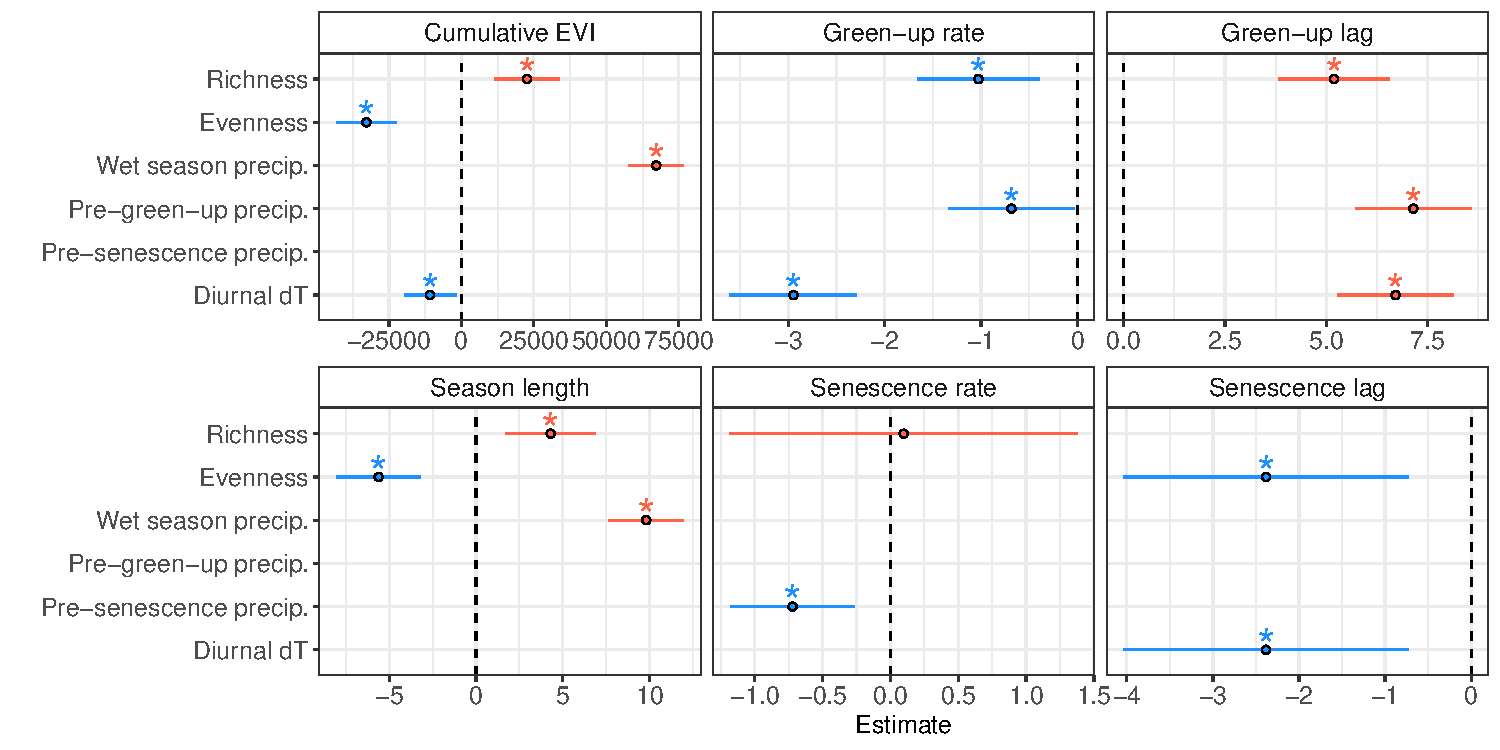
\includegraphics[width=\textwidth]{mod_slopes.pdf}
	\caption{Standardized slope coefficients for each best model of a phenological metric. Slope estimates are $\pm$1 standard error. Slope estimates where the interval does not overlap zero are considered to be significant effects and are marked by asterisks.}
	\label{mod_slopes}
\end{figure}

\begin{figure}[H]
\centering
	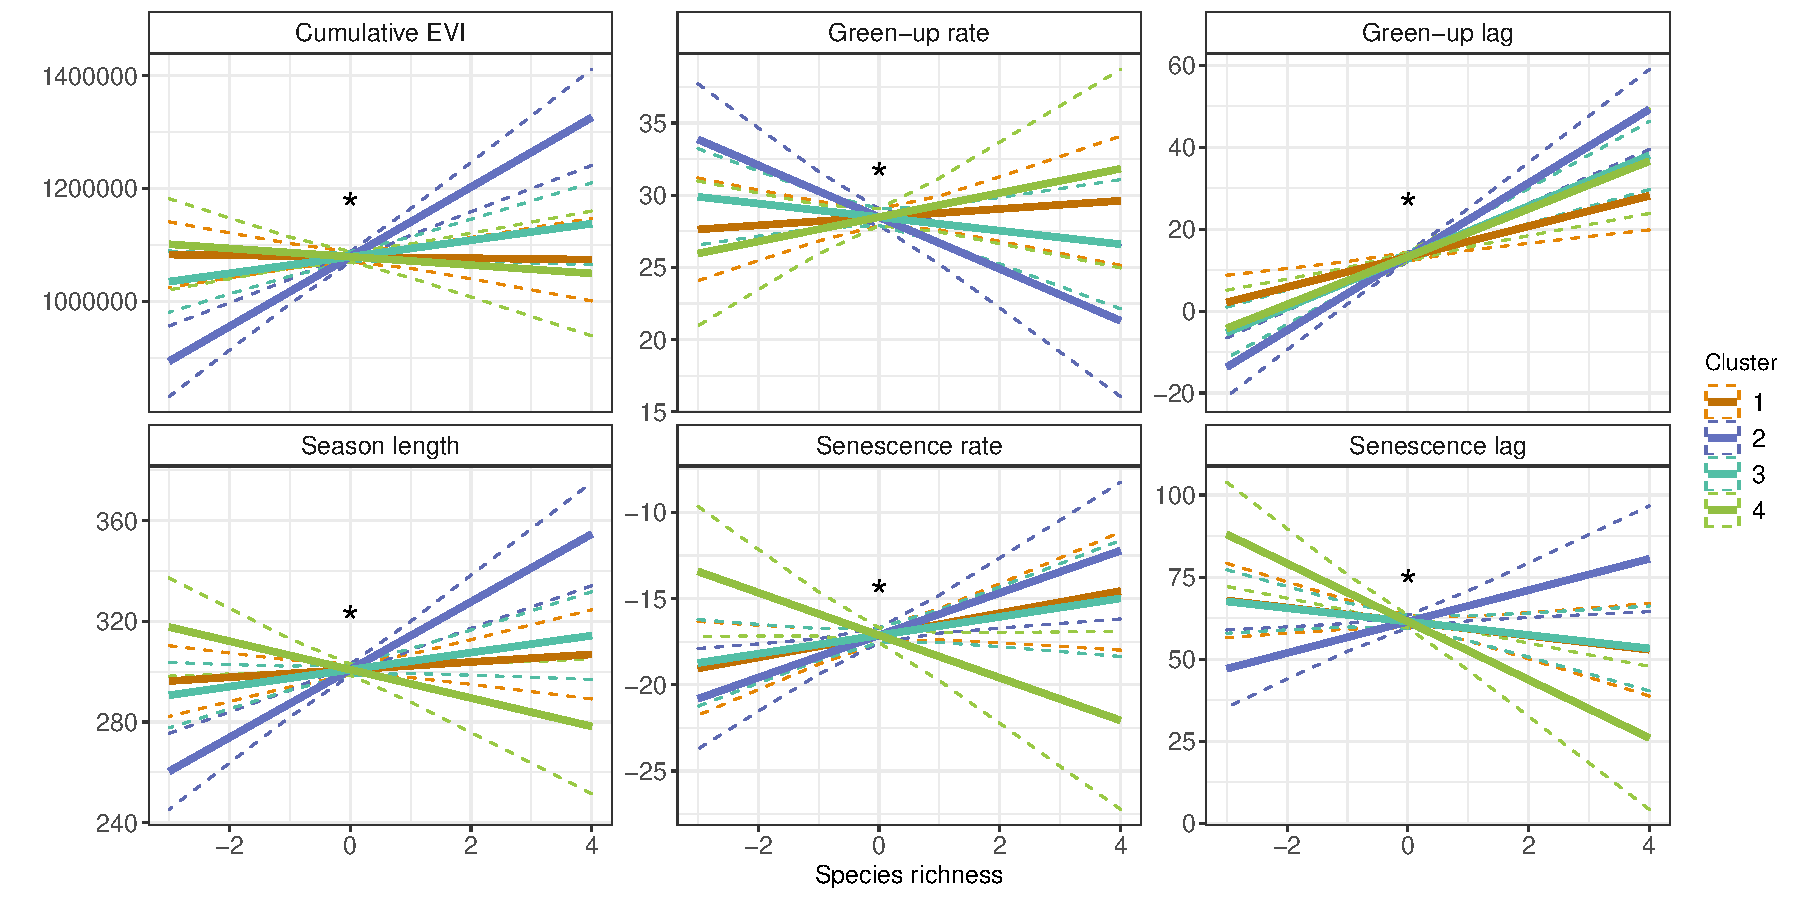
\includegraphics[width=\textwidth]{mod_marg.pdf}
	\caption{Marginal effects of tree species diversity on each of the phenological metrics, using the maximal mixed effects model, for each vegetation cluster. Dotted lines represent 95\% confidence intervals.}
	\label{mod_marg}
\end{figure}

\begin{figure}[H]
\centering
	\includegraphics[width=0.7\textwidth]{diam_quad_mod_slopes.pdf}
	\caption{Standardized slope coefficients for the fixed effect of average tree size on each phenological metric. Slope estimates are $\pm$1 standard error. Slope estimates where the interval does not overlap zero are considered to be significant effects and are marked by asterisks.}
	\label{diam_quad_mod_slopes}
\end{figure}

\begin{figure}[H]
\centering
	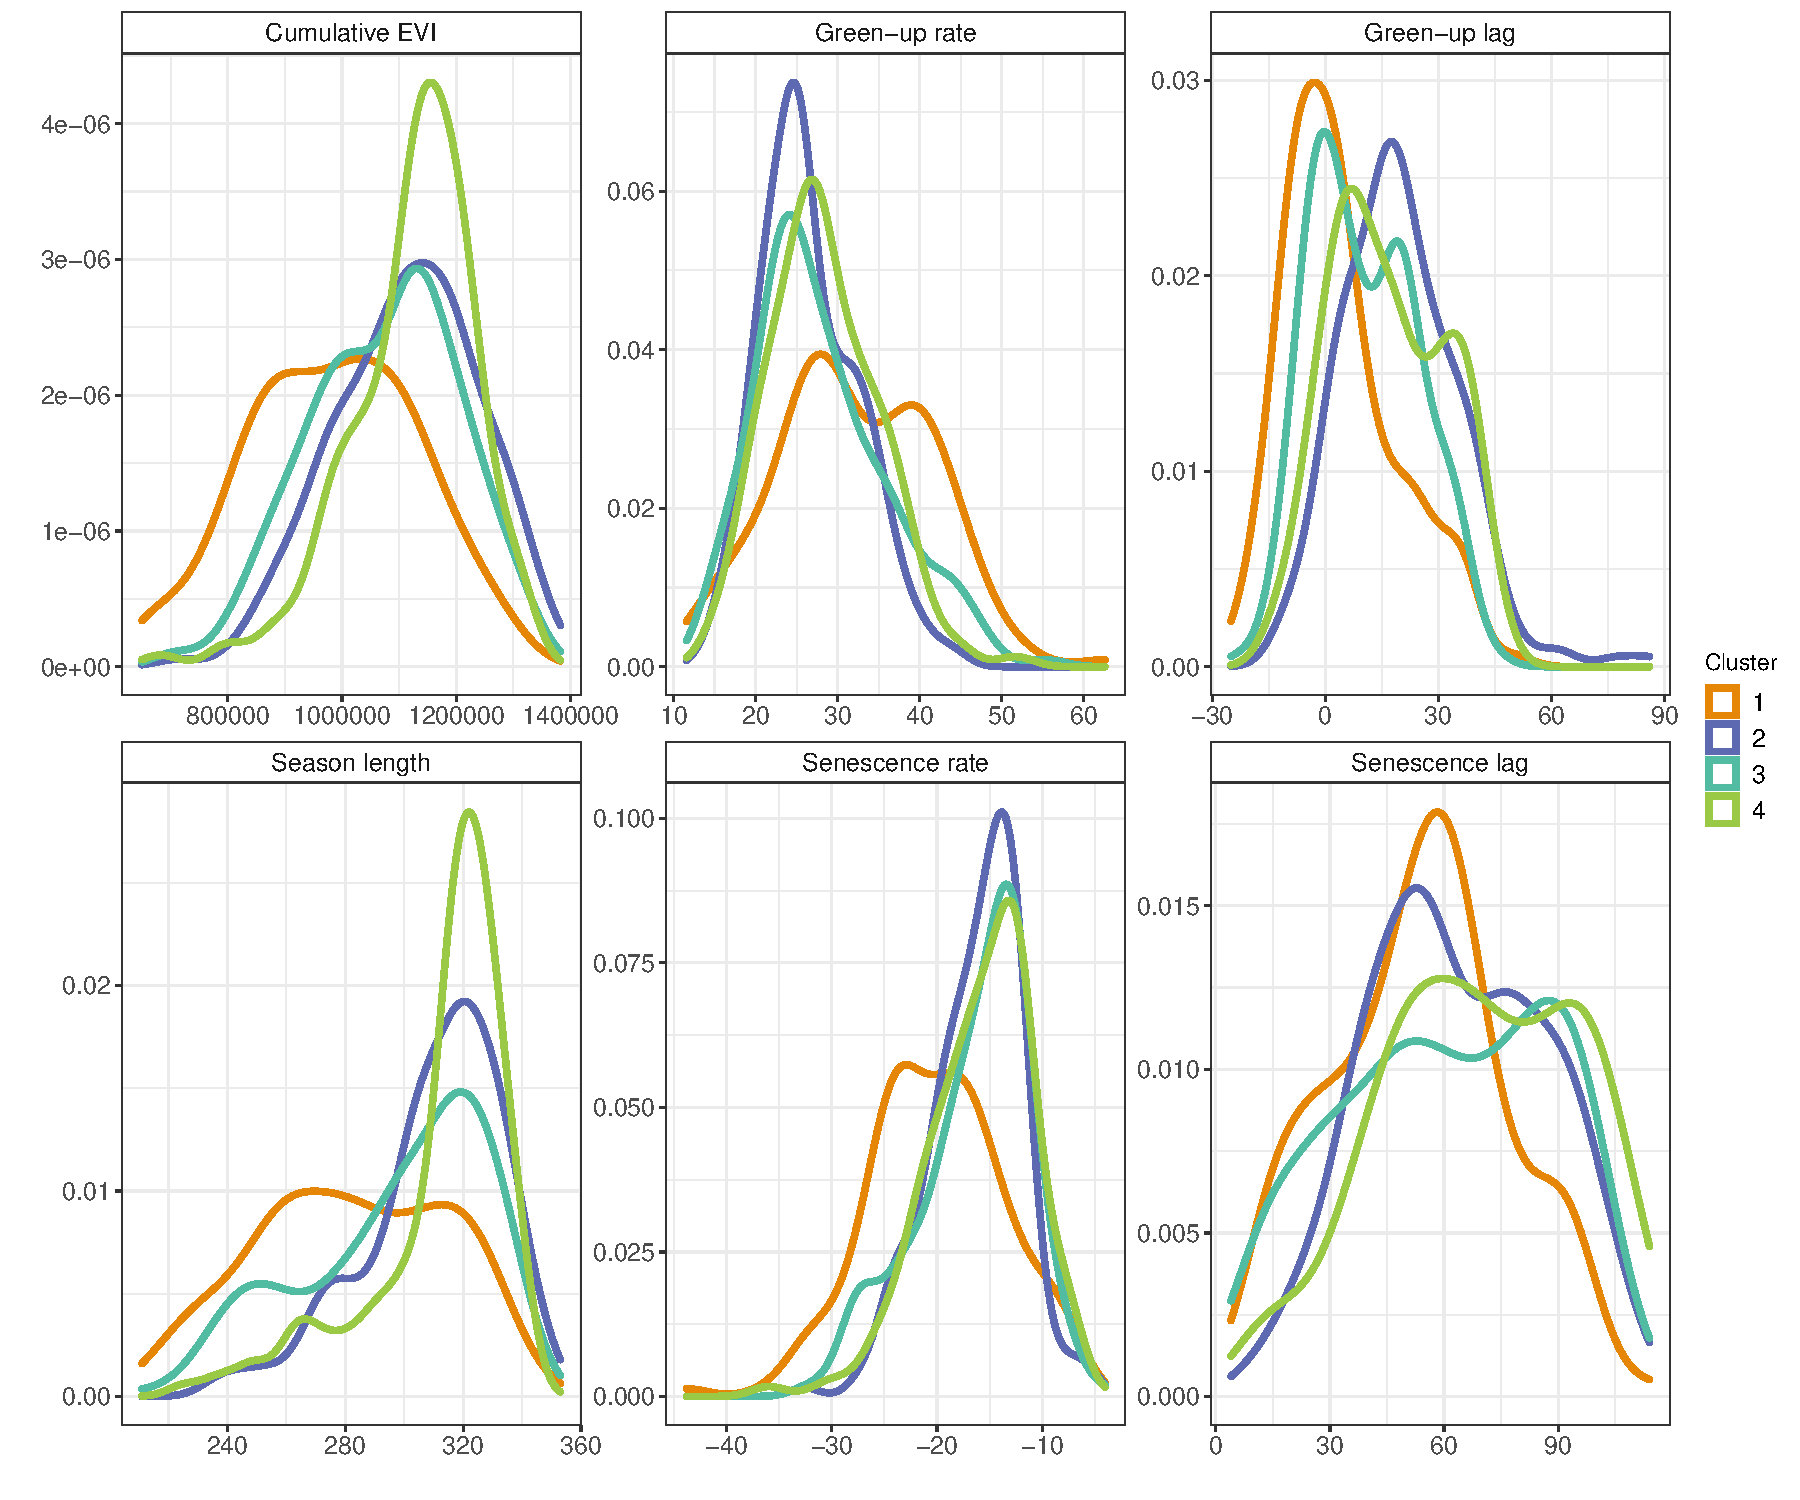
\includegraphics[width=\textwidth]{phen_dens_clust}
	\caption{Density distribution of the six phenological metrics used in the study, grouped by vegetation cluster.}
	\label{phen_dens_clust}
\end{figure}

\section{Discussion}

In this study we have demonstrated clear and measurable effects of tree species diversity, species composition, and woodland structure on various aspects of land-surface phenology in Zambian deciduous savannas. We showed that tree species diversity led to an increase in cumulative EVI and season length. Additionally, species diversity caused the onset of greening to occur earlier with respect to the start of the wet season. We also showed that woodlands comprising larger trees are able to maintain a longer growing season by allowing earlier pre-rain green-up, and by extending the end of the growing season. Our study lends support for a positive biodiversity - ecosystem function relationship in deciduous savannas, operating through its influence on phenology. Our results exemplify the role of tree species diversity as a driver of key ecosystem processes, which affect ecosystem structure, the wildlife provisioning role, and gross primary productivity.

Our finding that species diversity strongly affects patterns of land-surface phenology in deciduous Zambian woodlands provides earth surface system modellers with a means to better understand how future changes in species diversity and composition will affect land-surface phenology and therefore the carbon cycle. Incorporating predictions of biotic change into carbon cycling models has been slow, owing to large uncertainties in the effects of diversity on Gross Primary Productivity (GPP). Our study provides a link by demonstrating a strong positive relationship between species diversity and EVI, which itself drives GPP.

Patterns of senescence were poorly predicted by species diversity and evenness in our models. \citet{Cho2017} found that tree cover, measured by MODIS LAI data, had a significant effect on senescence rates in savannas in South Africa, which have similar climatic conditions to the sites in our study. In sparse savannas, while the onset of the growing season is often driven by tree photosynthetic activity, which may precede the onset of precipitation, the end of the growing season is conversely driven by the understorey grass layer, which can itself be dependent on tree cover \citep{Cho2017, Guan2014}. Grass activity is much more reactive to short-term changes in soil moisture than tree activity, and may oscillate within the senescence period. This may explain the lack of a strong precipitation signal for senescence lag and senescence rate in our models. 

Other studies both globally and within southern African savannas have largely ignored patterns of senescence, instead focussing patterns of green-up \citep{Gallinat2015}. Most commonly, these studies simply correlate the decline of rainfall with senescence, but our best model suggests that diurnal temperature range is a stronger determinant of the end of the growing season than precipitation. Alternatively, \citet{Zani2020} suggests that in resource limited environments, senescence times may largely be set by the preceding photosynthetic activity and sink-limitations on growth. For example, limited nutrient supply may prohibit photosynthesis late in the season if the preceding photosynthetic activity has depleted that supply. \citet{Reich1992} suggested that there may be direct constraints on leaf life-span, especially in disturbance and drought-prone environments such as those studied here, which would lead to senescence rate being set largely by the time since bud-burst. Our study corroborates this theory, showing that precipitation across the entire wet season was a better predictor of senescence lag than pre-senescence precipitation, while pre-senescence precipitation does cause variation in the rate of senescence. 

While leaf senescence may not be as important for the survival of browsing herbivores as the green-up period, the timing of senescence with respect to temperature and precipitation has important consequences for the savanna understorey microclimate. The longer leaf material remains in the canopy after the end of the wet season, the greater the microclimatic buffer for herbaceous understorey plants and animals, which require water and protection from high levels of insolation and dry air which can prevail rapidly after the end of the wet season \citep{Guan2014}. Our study merely exemplifies that more work needs to be done to properly characterise the drivers of senescence in this biome, which were poorly constrained in our models.

While species diversity is a common measure of biodiversity, abundance evenness constitutes a second key but related axis \citep{Wilsey2005, Hillebrand2008, Jost2010}. In this study, we found contrasting effects of diversity and evenness on cumulative EVI, season length and green-up lag. Evenness caused a decrease in these phenological metrics, which we did not expect. It is possible that the negative effect of abundance evenness occurred because an increase in evenness is associated with a reduction in the dominance of a few large canopy miombo tree species (e.g. \textit{Brachystegia boehmii} and \textit{Julbernardia paniculata}), as part of the transition from woody savanna to the thicket vegetation represented by vegetation Cluster 2. Large canopy tree species have access to groundwater for a longer part of the year, due to their deep root systems and conservative growth patterns. Indeed, our study found that plots with larger trees tend to green-up earlier and senesce later with respect to the start and end of the wet season. The effect of species diversity on cumulative EVI and season length was driven largely by the response of vegetation Cluster 2, which consisted of shorter stature non-miombo vegetation, while Clusters 1, 3 and 4, which consisted of miombo vegetation, exhibited negligible species diversity effects on these two phenological metrics. In miombo vegetation, it appears that dominant canopy forming tree species drive productivity through selection effects, while in the resource-limited scrubby vegetation represented by Cluster 2, a genuine species diversity effect driven by niche complementarity exists. 

Our coverage of very short growing season lengths in Zambia was restricted, with a notable absence of plot data in the northeast of the country around 30.5\textdegree{}E, 11.5\textdegree{}S, and 23.0\textdegree{}E, 15.0\textdegree{}S. Upon further inspection of true colour satellite imagery, these regions are largely seasonally water-logged floodplain and swampland, and were likely ignored by the ILUA-II assessment for this reason. This also explains their divergent phenological patterns as observed in the MODIS EVI data. While our study focusses on woodlands, the phenological behaviour of these other vegetation types should also be considered in future studies, as these may be even more sensitive to changes in climate \citep{Dean2018} and under greater land-use change pressures \citep{Langan2018}.

It is important to note that the remotely sensed EVI measurements used here aren't specific only to trees, they represent the landscape as a singe unit. Nevertheless, seasonal patterns of tree leaf phenology in southern African deciduous woodlands, particularly the pre-rain green-up phenomenon, is driven almost exclusively by trees, while grasses tend to follow patterns of precipitation more closely \citep{Whitecross2017, Archibald2007, Higgins2011}. Grasses contribute to gross primary productivity, and it was therefore in our interests to include their response in our analysis as we seek to demonstrate how tree species diversity can affect cycles of carbon exchange. Additionally, the micro-climatic effects of tree leaf canopy coverage and hydraulic lift through tree deep root systems will benefit the productivity of grasses as well as understorey tree individuals.

\section{Conclusion}

Here we explored the role of tree species diversity, composition and woodland structure on land surface phenology across Zambia. We showed that species diversity clearly affects the lag time between wet season onset and growth, the length of the growing season, and ultimately woodland productivity, as measured by cumulative EVI. We also demonstrated the effect of woodland demographic structure on land surface phenology, with woodlands consisting of larger trees maintaining a longer growing season, extending it beyond the wet season. Finally, we have demonstrated variation in phenological patterns among vegetation types within Zambia that are commonly not distinguished between in earth system models. Our results have a range of consequences for earth system modellers as well as conservation managers working in Zambia and across the dry tropics, and lend further support to an already well established corpus of the positive effect of species diversity on ecosystem function.

\printbibliography

\section{Supplementary Material}
\beginsupplement

\begin{figure}[H]
\centering
	\includegraphics[width=\textwidth]{vipphen_compare}
	\caption{Scatter plots showing a comparison of phenological metrics from the MODIS VIPPHEN product \citep{VIPPHEN} and those extracted from the MOD13Q1 data \citep{MOD13Q1}, for each of the sites in our study. The cyan line shows a linear model of the data, with a 95\% confidence interval.}
	\label{vipphen_compare}
\end{figure}

% latex table generated in R 4.0.2 by xtable 1.8-4 package
% Tue Mar 16 10:45:47 2021
\begin{table}[h]
\centering
\begin{tabular}{rcccc}
  \hline
Response & DoF & F & Prob. & R\textsuperscript{2} \\ 
  \hline
Mean EVI & 730 & 312.4 & p<0.05 & 0.30 \\ 
  Cumulative EVI & 730 & 635.2 & p<0.05 & 0.47 \\ 
  Season start & 730 & 568.7 & p<0.05 & 0.44 \\ 
  Season end & 730 & 279.4 & p<0.05 & 0.28 \\ 
  Season length & 730 & 408.0 & p<0.05 & 0.36 \\ 
  Green-up rate & 730 & 288.9 & p<0.05 & 0.28 \\ 
  Senescence rate & 730 & 408.2 & p<0.05 & 0.36 \\ 
   \hline
\end{tabular}
\caption{Model fit statistics for comparison of MODIS VIPPHEN and MOD13Q1 products across each of our study sites.} 
\label{annot_df}
\end{table}



\begin{figure}[H]
\centering
	\includegraphics[width=\textwidth]{phen_bivar}
	\caption{Scatter plots showing pairwise comparisons of the six phenological metrics used in this study, extracted from the MODIS MOD13Q1 product \citep{MOD13Q1}. Points represent study sites and are coloured by vegetation cluster. Linear regression line of best fit for all sites is shown as a black line, while linear regressions are shown for each vegetation cluster as coloured lines.}
	\label{phen_bivar}
\end{figure}

% latex table generated in R 4.0.2 by xtable 1.8-4 package
% Tue Oct 27 08:49:06 2020
\begin{table}[ht]
\centering
\begin{tabular}{cccccrrrr}
  \hline
Rank & Precipitation & Diurnal dT & Evenness & Richness & logLik & AIC & $\Delta{}IC$ & $W_{i}$ \\ 
  \hline
1 & \checkmark & \checkmark & \checkmark & \checkmark & -5933 & 11885 & 0.00 & 0.333 \\ 
  2 & \checkmark & \checkmark & \checkmark & \checkmark & -5935 & 11885 & 0.21 & 0.299 \\ 
  3 & \checkmark & \checkmark &  & \checkmark & -5937 & 11887 & 2.08 & 0.118 \\ 
  4 & \checkmark & \checkmark & \checkmark &  & -5937 & 11887 & 2.14 & 0.115 \\ 
  5 & \checkmark & \checkmark &  & \checkmark & -5935 & 11887 & 2.31 & 0.105 \\ 
  6 & \checkmark & \checkmark &  &  & -5940 & 11890 & 4.77 & 0.031 \\ 
  7 &  & \checkmark & \checkmark &  & -5947 & 11904 & 18.38 & 0.000 \\ 
  8 &  & \checkmark &  &  & -5948 & 11905 & 20.15 & 0.000 \\ 
  9 &  & \checkmark & \checkmark & \checkmark & -5946 & 11905 & 20.26 & 0.000 \\ 
  10 &  & \checkmark & \checkmark & \checkmark & -5945 & 11906 & 20.99 & 0.000 \\ 
   \hline
\end{tabular}
\caption{Cumulative EVI model selection candidate models, with fit statistics.} 
\label{mod_sel_cum_vi}
\end{table}

% latex table generated in R 4.0.2 by xtable 1.8-4 package
% Tue Oct 27 08:49:07 2020
\begin{table}[ht]
\centering
\begin{tabular}{cccccrrrr}
  \hline
Rank & Precipitation & Diurnal dT & Evenness & Richness & logLik & AIC & $\Delta{}IC$ & $W_{i}$ \\ 
  \hline
1 & \checkmark & \checkmark &  & \checkmark & -3041 & 6094 & 0.00 & 0.346 \\ 
  2 & \checkmark & \checkmark &  & \checkmark & -3039 & 6094 & 0.05 & 0.338 \\ 
  3 & \checkmark & \checkmark & \checkmark & \checkmark & -3039 & 6096 & 1.53 & 0.161 \\ 
  4 & \checkmark & \checkmark & \checkmark & \checkmark & -3041 & 6096 & 1.63 & 0.153 \\ 
  5 &  & \checkmark &  & \checkmark & -3046 & 6107 & 13.27 & 0.000 \\ 
  6 &  & \checkmark &  & \checkmark & -3048 & 6107 & 13.28 & 0.000 \\ 
  7 &  & \checkmark & \checkmark & \checkmark & -3046 & 6109 & 14.93 & 0.000 \\ 
  8 &  & \checkmark & \checkmark & \checkmark & -3048 & 6109 & 15.04 & 0.000 \\ 
  9 & \checkmark & \checkmark &  &  & -3059 & 6128 & 34.02 & 0.000 \\ 
  10 & \checkmark & \checkmark & \checkmark &  & -3058 & 6129 & 34.77 & 0.000 \\ 
   \hline
\end{tabular}
\caption{Senescence lag model selection candidate models, with fit statistics.} 
\label{mod_sel_end_lag}
\end{table}

% latex table generated in R 4.0.2 by xtable 1.8-4 package
% Tue Oct 27 08:49:07 2020
\begin{table}[ht]
\centering
\begin{tabular}{cccccrrrr}
  \hline
Rank & Precipitation & Diurnal dT & Evenness & Richness & logLik & AIC & $\Delta{}IC$ & $W_{i}$ \\ 
  \hline
1 & \checkmark & \checkmark &  & \checkmark & 881 & -1751 & 0.00 & 0.369 \\ 
  2 & \checkmark & \checkmark & \checkmark & \checkmark & 881 & -1749 & 1.35 & 0.188 \\ 
  3 & \checkmark & \checkmark &  & \checkmark & 882 & -1749 & 1.91 & 0.142 \\ 
  4 &  & \checkmark &  & \checkmark & 879 & -1748 & 2.88 & 0.087 \\ 
  5 & \checkmark & \checkmark & \checkmark & \checkmark & 883 & -1748 & 3.05 & 0.080 \\ 
  6 &  & \checkmark & \checkmark & \checkmark & 879 & -1746 & 4.45 & 0.040 \\ 
  7 &  & \checkmark &  & \checkmark & 880 & -1746 & 4.89 & 0.032 \\ 
  8 & \checkmark & \checkmark &  &  & 877 & -1745 & 5.46 & 0.024 \\ 
  9 & \checkmark & \checkmark & \checkmark &  & 878 & -1744 & 6.28 & 0.016 \\ 
  10 &  & \checkmark & \checkmark & \checkmark & 880 & -1744 & 6.29 & 0.016 \\ 
   \hline
\end{tabular}
\caption{Green-up rate model selection candidate models, with fit statistics.} 
\label{mod_sel_s1_green_rate}
\end{table}

% latex table generated in R 4.0.2 by xtable 1.8-4 package
% Tue Oct 27 08:49:07 2020
\begin{table}[ht]
\centering
\begin{tabular}{cccccrrrr}
  \hline
Rank & Precipitation & Diurnal dT & Evenness & Richness & logLik & AIC & $\Delta{}IC$ & $W_{i}$ \\ 
  \hline
1 & \checkmark &  & \checkmark & \checkmark & -2966 & 5945 & 0.00 & 0.448 \\ 
  2 & \checkmark & \checkmark & \checkmark & \checkmark & -2966 & 5946 & 1.43 & 0.220 \\ 
  3 & \checkmark &  & \checkmark & \checkmark & -2965 & 5947 & 2.08 & 0.158 \\ 
  4 & \checkmark & \checkmark & \checkmark & \checkmark & -2965 & 5948 & 3.53 & 0.077 \\ 
  5 & \checkmark &  & \checkmark &  & -2969 & 5949 & 3.96 & 0.062 \\ 
  6 & \checkmark & \checkmark & \checkmark &  & -2969 & 5950 & 5.69 & 0.026 \\ 
  7 & \checkmark &  &  & \checkmark & -2972 & 5954 & 9.49 & 0.004 \\ 
  8 & \checkmark & \checkmark &  & \checkmark & -2971 & 5955 & 10.67 & 0.002 \\ 
  9 & \checkmark &  &  & \checkmark & -2971 & 5957 & 11.90 & 0.001 \\ 
  10 & \checkmark &  &  &  & -2974 & 5957 & 11.92 & 0.001 \\ 
   \hline
\end{tabular}
\caption{Season length model selection candidate models, with fit statistics.} 
\label{mod_sel_s1_length}
\end{table}

% latex table generated in R 4.0.2 by xtable 1.8-4 package
% Tue Oct 27 08:49:07 2020
\begin{table}[ht]
\centering
\begin{tabular}{cccccrrrr}
  \hline
Rank & Precipitation & Diurnal dT & Evenness & Richness & logLik & AIC & $\Delta{}IC$ & $W_{i}$ \\ 
  \hline
1 & \checkmark & \checkmark &  & \checkmark & 1245 & -2474 & 0.00 & 0.449 \\ 
  2 & \checkmark &  &  & \checkmark & 1243 & -2472 & 1.70 & 0.192 \\ 
  3 & \checkmark & \checkmark & \checkmark & \checkmark & 1245 & -2472 & 1.80 & 0.182 \\ 
  4 & \checkmark &  & \checkmark & \checkmark & 1243 & -2470 & 3.56 & 0.076 \\ 
  5 & \checkmark & \checkmark &  & \checkmark & 1240 & -2469 & 4.63 & 0.044 \\ 
  6 & \checkmark &  &  & \checkmark & 1239 & -2468 & 5.98 & 0.023 \\ 
  7 & \checkmark & \checkmark & \checkmark & \checkmark & 1240 & -2467 & 6.51 & 0.017 \\ 
  8 & \checkmark &  & \checkmark & \checkmark & 1239 & -2466 & 7.92 & 0.009 \\ 
  9 & \checkmark &  &  &  & 1236 & -2464 & 10.04 & 0.003 \\ 
  10 & \checkmark & \checkmark &  &  & 1237 & -2464 & 10.16 & 0.003 \\ 
   \hline
\end{tabular}
\caption{Senescence rate model selection candidate models, with fit statistics.} 
\label{mod_sel_s1_senes_rate}
\end{table}

% latex table generated in R 4.0.2 by xtable 1.8-4 package
% Tue Oct 27 08:49:07 2020
\begin{table}[ht]
\centering
\begin{tabular}{cccccrrrr}
  \hline
Rank & Precipitation & Diurnal dT & Evenness & Richness & logLik & AIC & $\Delta{}IC$ & $W_{i}$ \\ 
  \hline
1 & \checkmark & \checkmark & \checkmark & \checkmark & -3074 & 6167 & 0.00 & 0.563 \\ 
  2 & \checkmark & \checkmark &  & \checkmark & -3076 & 6168 & 1.63 & 0.249 \\ 
  3 & \checkmark & \checkmark & \checkmark & \checkmark & -3077 & 6169 & 2.85 & 0.135 \\ 
  4 & \checkmark & \checkmark &  & \checkmark & -3079 & 6171 & 4.72 & 0.053 \\ 
  5 & \checkmark & \checkmark &  &  & -3102 & 6215 & 48.86 & 0.000 \\ 
  6 & \checkmark & \checkmark & \checkmark &  & -3102 & 6216 & 49.48 & 0.000 \\ 
  7 &  & \checkmark & \checkmark & \checkmark & -3130 & 6273 & 106.35 & 0.000 \\ 
  8 &  & \checkmark & \checkmark & \checkmark & -3128 & 6273 & 106.77 & 0.000 \\ 
  9 &  & \checkmark &  & \checkmark & -3133 & 6277 & 110.46 & 0.000 \\ 
  10 &  & \checkmark &  & \checkmark & -3131 & 6277 & 110.63 & 0.000 \\ 
   \hline
\end{tabular}
\caption{Green-up lag model selection candidate models, with fit statistics.} 
\label{mod_sel_start_lag}
\end{table}



\renewcommand{\arraystretch}{0.8}
% latex table generated in R 4.0.2 by xtable 1.8-4 package
% Fri Oct 30 14:34:06 2020
\begin{table}[H]
\centering
\begin{tabular}{rcccccc}
  \hline
Response & Clusters & Estimate & SE & DoF & T ratio & Prob. \\ 
  \hline
Cumulative EVI & 1-2 & 1.1E-14 & 6.68E-14 & 697 & 0.17 & 0.98 \\ 
  Cumulative EVI & 1-3 & 5.5E-14 & 6.33E-14 & 697 & 0.87 & 0.66 \\ 
  Cumulative EVI & 2-3 & 4.4E-14 & 8.16E-14 & 697 & 0.54 & 0.85 \\ 
   \hline
Season length & 1-2 & -6.4E-18 & 1.56E-17 & 698 & -0.41 & 0.91 \\ 
  Season length & 1-3 & 1.9E-17 & 1.48E-17 & 698 & 1.26 & 0.42 \\ 
  Season length & 2-3 & 2.5E-17 & 1.89E-17 & 698 & 1.32 & 0.38 \\ 
   \hline
Green-up rate & 1-2 & 1.1E-18 & 4.89E-18 & 698 & 0.23 & 0.97 \\ 
  Green-up rate & 1-3 & -3.5E-18 & 4.59E-18 & 698 & -0.76 & 0.73 \\ 
  Green-up rate & 2-3 & -4.6E-18 & 5.91E-18 & 698 & -0.78 & 0.72 \\ 
   \hline
Senescence rate & 1-2 & 3.7E-18 & 3.41E-18 & 698 & 1.09 & 0.52 \\ 
  Senescence rate & 1-3 & 6.3E-18 & 3.21E-18 & 698 & 1.97 & 0.12 \\ 
  Senescence rate & 2-3 & 2.6E-18 & 4.14E-18 & 698 & 0.63 & 0.80 \\ 
   \hline
Green-up lag & 1-2 & -7.3E-18 & 1.03E-17 & 698 & -0.71 & 0.76 \\ 
  Green-up lag & 1-3 & 6.0E-18 & 9.71E-18 & 698 & 0.62 & 0.81 \\ 
  Green-up lag & 2-3 & 1.3E-17 & 1.25E-17 & 698 & 1.07 & 0.54 \\ 
   \hline
Senescence lag & 1-2 & 2.9E-19 & 1.30E-17 & 698 & 0.02 & 1.00 \\ 
  Senescence lag & 1-3 & 6.1E-18 & 1.23E-17 & 698 & 0.50 & 0.87 \\ 
  Senescence lag & 2-3 & 5.9E-18 & 1.59E-17 & 698 & 0.37 & 0.93 \\ 
  \end{tabular}
\caption{Comparisons of interaction marginal effects using post-hoc Tukey's tests.} 
\label{lsq_terms}
\end{table}



% latex table generated in R 4.1.0 by xtable 1.8-4 package
% Fri Jul 16 12:26:46 2021
\begin{table}[H]
\centering
\begin{tabular}{rcccc}
  \hline
Response & Clusters & Mean diff. & Interval & Prob. \\ 
  \hline
 & 2-1 & -0.77 & -1.05 - -0.5 & p<0.01 \\ 
   & 3-1 & -0.09 & -0.34 - 0.15 & p = 0.76 \\ 
  Cumulative EVI & 4-1 &  0.13 & -0.18 - 0.44 & p = 0.72 \\ 
   & 3-2 &  0.68 & 0.43 - 0.93 & p<0.01 \\ 
   & 4-2 &   0.9 & 0.59 - 1.21 & p<0.01 \\ 
   & 4-3 &  0.22 & -0.07 - 0.51 & p = 0.20 \\ 
   \hline
 & 2-1 & -0.63 & -0.9 - -0.36 & p<0.01 \\ 
   & 3-1 &  0.17 & -0.07 - 0.42 & p = 0.26 \\ 
  Season length & 4-1 &  0.32 & 0.01 - 0.63 & p<0.05 \\ 
   & 3-2 &   0.8 & 0.56 - 1.05 & p<0.01 \\ 
   & 4-2 &  0.95 & 0.64 - 1.26 & p<0.01 \\ 
   & 4-3 &  0.15 & -0.14 - 0.43 & p = 0.54 \\ 
   \hline
 & 2-1 &  0.27 & -0.01 - 0.55 & p = 0.06 \\ 
   & 3-1 & -0.43 & -0.68 - -0.19 & p<0.01 \\ 
  Green-up rate & 4-1 & -0.45 & -0.77 - -0.14 & p<0.01 \\ 
   & 3-2 &  -0.7 & -0.95 - -0.45 & p<0.01 \\ 
   & 4-2 & -0.72 & -1.04 - -0.41 & p<0.01 \\ 
   & 4-3 & -0.02 & -0.31 - 0.27 & p = 1.00 \\ 
   \hline
 & 2-1 & -0.62 & -0.89 - -0.35 & p<0.01 \\ 
   & 3-1 &  0.12 & -0.12 - 0.36 & p = 0.58 \\ 
  Senescence rate & 4-1 &  0.55 & 0.25 - 0.86 & p<0.01 \\ 
   & 3-2 &  0.74 & 0.49 - 0.98 & p<0.01 \\ 
   & 4-2 &  1.17 & 0.86 - 1.48 & p<0.01 \\ 
   & 4-3 &  0.43 & 0.15 - 0.72 & p<0.01 \\ 
   \hline
 & 2-1 & -0.49 & -0.77 - -0.21 & p<0.01 \\ 
   & 3-1 &  0.32 & 0.07 - 0.57 & p<0.01 \\ 
  Green-up lag & 4-1 &  0.14 & -0.18 - 0.45 & p = 0.67 \\ 
   & 3-2 &  0.81 & 0.56 - 1.06 & p<0.01 \\ 
   & 4-2 &  0.63 & 0.31 - 0.94 & p<0.01 \\ 
   & 4-3 & -0.18 & -0.47 - 0.11 & p = 0.38 \\ 
   \hline
 & 2-1 & -0.25 & -0.54 - 0.03 & p = 0.10 \\ 
   & 3-1 &  0.13 & -0.13 - 0.39 & p = 0.57 \\ 
  Senescence lag & 4-1 &   0.2 & -0.13 - 0.52 & p = 0.41 \\ 
   & 3-2 &  0.38 & 0.13 - 0.64 & p<0.01 \\ 
   & 4-2 &  0.45 & 0.12 - 0.78 & p<0.01 \\ 
   & 4-3 &  0.07 & -0.23 - 0.37 & p = 0.94 \\ 
   \hline
\end{tabular}
\caption{Post-hoc Tukey's pairwise comparisons among vegetation types for each phenological metric.} 
\label{tukey_terms}
\end{table}



\end{document}

